\section{Methods}

\subsection{Overview}

Our goal is to build and compare two deep learning models a Deep Neural Network (DNN) and a Convolutional Neural Network (CNN) for predicting loan approval based on multi-modal inputs: tabular financial features and free-text loan descriptions. Both models share a common text processing branch powered by BERT, while the tabular processing branch differs. The final predictions are made by fusing the outputs from both modalities.

\begin{figure}[h]
    \centering
    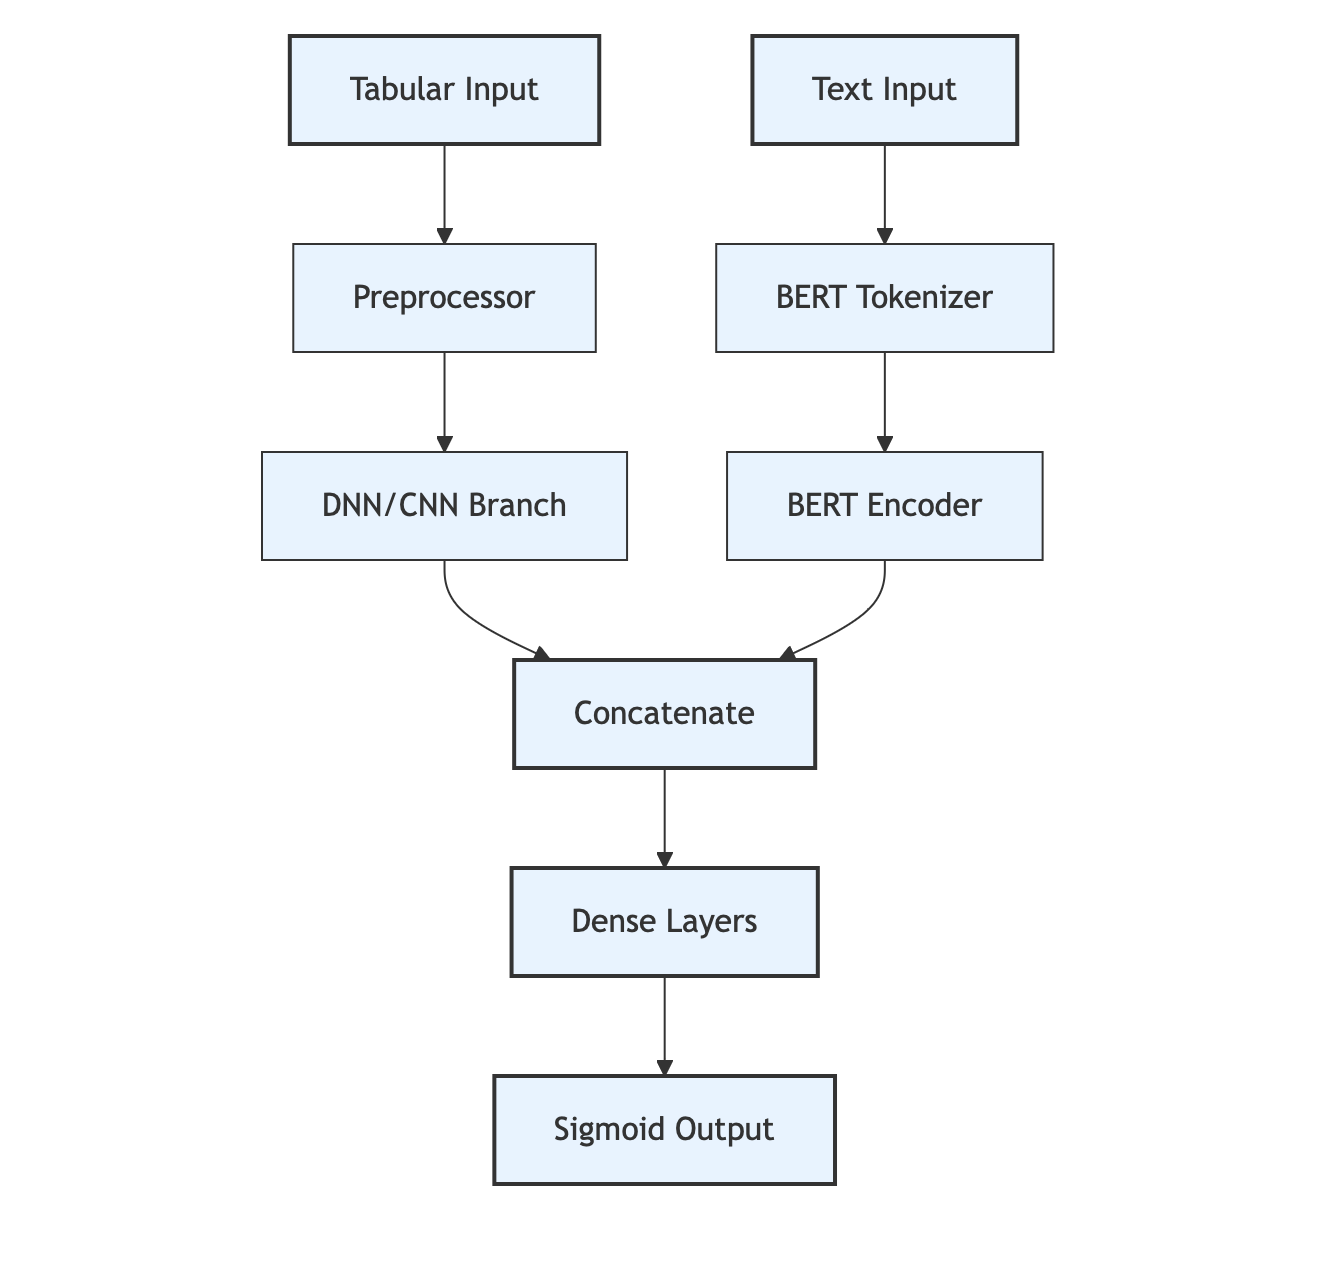
\includegraphics[width=0.85\linewidth]{figures/project_flowchart.png}
    \caption{Multi-modal pipeline combining tabular and textual inputs using a shared BERT encoder and DNN/CNN branch for binary loan prediction.}
    
    \label{fig:flowchart}
\end{figure}

\subsection{Tabular Input Processing}

The dataset includes numerical and categorical financial attributes. We use a \texttt{ColumnTransformer} to apply \texttt{StandardScaler} on numerical features and \texttt{OneHotEncoder} on categorical ones. This transformation is applied consistently across both models.

\subsection{Text Input Processing}

For textual input, we combine the loan \texttt{purpose} and \texttt{title} fields. The combined text is tokenized using the pre-trained \texttt{bert-base-uncased} tokenizer, and passed through a frozen BERT encoder. We extract the pooled [CLS] representation (768-dimensional) as the final output from the text branch.

\subsection{DNN Architecture}

The tabular branch of the DNN model consists of two dense layers:
\begin{itemize}
    \item \texttt{Dense(64) → ReLU → Dropout(0.3)}
    \item \texttt{Dense(32) → ReLU}
\end{itemize}

The BERT output and tabular features are concatenated and passed through:
\begin{itemize}
    \item \texttt{Dense(64) → ReLU → Dropout(0.3)}
    \item \texttt{Dense(1) → Sigmoid (binary classification)}
\end{itemize}

\subsection{CNN Architecture}

The CNN model uses the same BERT text branch, but processes tabular features using 1D convolutions:
\begin{itemize}
    \item \texttt{Conv1D(64, kernel\_size=3, padding='same') → ReLU}
    \item \texttt{Conv1D(32, kernel\_size=3, padding='same') → ReLU}
    \item \texttt{GlobalMaxPooling → Dense(32) → ReLU}
\end{itemize}

The tabular CNN output is concatenated with the BERT embedding and passed through:
\begin{itemize}
    \item \texttt{Dense(64) → ReLU → Dropout(0.3)}
    \item \texttt{Dense(1) → Sigmoid}
\end{itemize}

\subsection{Training Details}

Both models were trained using the following configuration:
\begin{itemize}
    \item \textbf{Loss Function:} Binary Cross-Entropy
    \item \textbf{Optimizer:} Adam
    \item \textbf{Batch Size:} 32
    \item \textbf{Early Stopping:} Patience = 3, restore best weights
    \item \textbf{Epochs:} Max = 10 (DNN stopped at 6, CNN at 5)
    \item \textbf{Hardware:} Google Colab Pro with high-RAM GPU
\end{itemize}

The training, validation, and test splits follow a 60/20/20 stratified split.